\documentclass[man]{apa6}

\usepackage{amssymb,amsmath}
\usepackage{ifxetex,ifluatex}
\usepackage{fixltx2e} % provides \textsubscript
\ifnum 0\ifxetex 1\fi\ifluatex 1\fi=0 % if pdftex
  \usepackage[T1]{fontenc}
  \usepackage[utf8]{inputenc}
\else % if luatex or xelatex
  \ifxetex
    \usepackage{mathspec}
    \usepackage{xltxtra,xunicode}
  \else
    \usepackage{fontspec}
  \fi
  \defaultfontfeatures{Mapping=tex-text,Scale=MatchLowercase}
  \newcommand{\euro}{€}
\fi
% use upquote if available, for straight quotes in verbatim environments
\IfFileExists{upquote.sty}{\usepackage{upquote}}{}
% use microtype if available
\IfFileExists{microtype.sty}{\usepackage{microtype}}{}

% Table formatting
\usepackage{longtable, booktabs}
\usepackage{lscape}
% \usepackage[counterclockwise]{rotating}   % Landscape page setup for large tables
\usepackage{multirow}		% Table styling
\usepackage{tabularx}		% Control Column width
\usepackage[flushleft]{threeparttable}	% Allows for three part tables with a specified notes section
\usepackage{threeparttablex}            % Lets threeparttable work with longtable

% Create new environments so endfloat can handle them
% \newenvironment{ltable}
%   {\begin{landscape}\begin{center}\begin{threeparttable}}
%   {\end{threeparttable}\end{center}\end{landscape}}

\newenvironment{lltable}
  {\begin{landscape}\begin{center}\begin{ThreePartTable}}
  {\end{ThreePartTable}\end{center}\end{landscape}}

  \usepackage{ifthen} % Only add declarations when endfloat package is loaded
  \ifthenelse{\equal{\string man}{\string man}}{%
   \DeclareDelayedFloatFlavor{ThreePartTable}{table} % Make endfloat play with longtable
   % \DeclareDelayedFloatFlavor{ltable}{table} % Make endfloat play with lscape
   \DeclareDelayedFloatFlavor{lltable}{table} % Make endfloat play with lscape & longtable
  }{}%



% The following enables adjusting longtable caption width to table width
% Solution found at http://golatex.de/longtable-mit-caption-so-breit-wie-die-tabelle-t15767.html
\makeatletter
\newcommand\LastLTentrywidth{1em}
\newlength\longtablewidth
\setlength{\longtablewidth}{1in}
\newcommand\getlongtablewidth{%
 \begingroup
  \ifcsname LT@\roman{LT@tables}\endcsname
  \global\longtablewidth=0pt
  \renewcommand\LT@entry[2]{\global\advance\longtablewidth by ##2\relax\gdef\LastLTentrywidth{##2}}%
  \@nameuse{LT@\roman{LT@tables}}%
  \fi
\endgroup}


\ifxetex
  \usepackage[setpagesize=false, % page size defined by xetex
              unicode=false, % unicode breaks when used with xetex
              xetex]{hyperref}
\else
  \usepackage[unicode=true]{hyperref}
\fi
\hypersetup{breaklinks=true,
            pdfauthor={},
            pdftitle={The title},
            colorlinks=true,
            citecolor=blue,
            urlcolor=blue,
            linkcolor=black,
            pdfborder={0 0 0}}
\urlstyle{same}  % don't use monospace font for urls

\setlength{\parindent}{0pt}
%\setlength{\parskip}{0pt plus 0pt minus 0pt}

\setlength{\emergencystretch}{3em}  % prevent overfull lines


% Manuscript styling
\captionsetup{font=singlespacing,justification=justified}
\usepackage{csquotes}
\usepackage{upgreek}

 % Line numbering
  \usepackage{lineno}
  \linenumbers


\usepackage{tikz} % Variable definition to generate author note

% fix for \tightlist problem in pandoc 1.14
\providecommand{\tightlist}{%
  \setlength{\itemsep}{0pt}\setlength{\parskip}{0pt}}

% Essential manuscript parts
  \title{The title}

  \shorttitle{Title}


  \author{First Author\textsuperscript{1}, Second Author\textsuperscript{1}, \& Third Author\textsuperscript{1}}

  % \def\affdep{{"", "", ""}}%
  % \def\affcity{{"", "", ""}}%

  \affiliation{
    \vspace{0.5cm}
          \textsuperscript{1} Stanford University  }

  \authornote{
    Add complete departmental affiliations for each author here. Each new
    line herein must be indented, like this line.
    
    Enter author note here.
    
    Correspondence concerning this article should be addressed to First
    Author, Postal address. E-mail:
    \href{mailto:my@email.com}{\nolinkurl{my@email.com}}
  }


  \abstract{Enter abstract here. Each new line herein must be indented, like this
line.}
  \keywords{keywords \\

    \indent Word count: X
  }





\usepackage{amsthm}
\newtheorem{theorem}{Theorem}
\newtheorem{lemma}{Lemma}
\theoremstyle{definition}
\newtheorem{definition}{Definition}
\newtheorem{corollary}{Corollary}
\newtheorem{proposition}{Proposition}
\theoremstyle{definition}
\newtheorem{example}{Example}
\theoremstyle{definition}
\newtheorem{exercise}{Exercise}
\theoremstyle{remark}
\newtheorem*{remark}{Remark}
\newtheorem*{solution}{Solution}
\begin{document}

\maketitle

\setcounter{secnumdepth}{0}



\section{Introduction}\label{introduction}

\section{Background}\label{background}

\begin{itemize}
\tightlist
\item
  discussing the ways people in tha past have measured the
  \enquote{implicature rate}.
\end{itemize}

\section{Methods}\label{methods}

\begin{itemize}
\tightlist
\item
  data exclusion? we don't expect any.
\end{itemize}

\subsection{Participants}\label{participants}

\begin{itemize}
\tightlist
\item
  how are we choosing the sample size?
\end{itemize}

\subsection{Materials and Design}\label{materials-and-design}

\begin{figure}[t]

{\centering 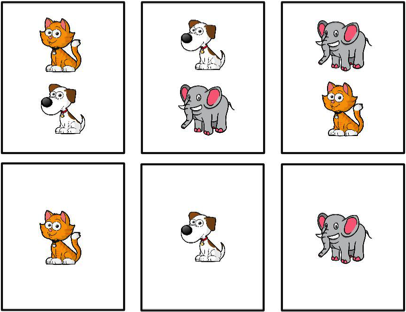
\includegraphics{writeup_files/figure-latex/stimuli-1} 

}

\caption{Cards used in the connective guessing game.}\label{fig:stimuli}
\end{figure}

\begin{itemize}
\tightlist
\item
  Manipulations: type of card and the type ofgue
\end{itemize}

The study included six cards with cartoon images of a cat, a dog, and an
elephant (Figure \ref{fig:stimuli}). The study was designed based on the
type of cards participants saw and the type of guesses they heard. There
were two types of cards: cards with only one animal on them and the ones
with two animals. There were three types of guesses: simple (e.g.
\emph{There is a cat}), conjunctive (e.g. \emph{There is a cat and a
dog}), and disjunctive (e.g. \emph{There is a cat or a dog}). In each
guess, the animal labels used in the guess and the animal images on the
card may have no overlap (e.g.~Image: dog, Guess: \emph{There is a cat
or an elephant}), a partial overlap (e.g.~Image: Cat, Guess: \emph{There
is a cat or an elephant}), or a total overlap (e.g.~Image: cat and
elephant, Guess: \emph{There is a cat or an elephant}). Crossing the
number of animals on the card, the type of guess, and the overlap
between the guess and the card results in 12 different possible trial
types. We chose 8 trial types (Figure \ref{fig:trials}), balancing the
number of one-animal vs.~two-animal cards, simple vs.~connective
guesses, and expected true vs.~false trials.

\begin{itemize}
\tightlist
\item
  The study used five different types of measurements. 1. two-options
  (true vs.~false) 2. two-options (wrong vs.~right) 3. three-options
  (wrong, neither, right) 4. four-options (wrong, kinda wrong, kinda
  right, right) 5. five-options (wrong, kinda wrong, neither, kinda
  right).
\end{itemize}

\begin{figure}[t]

{\centering 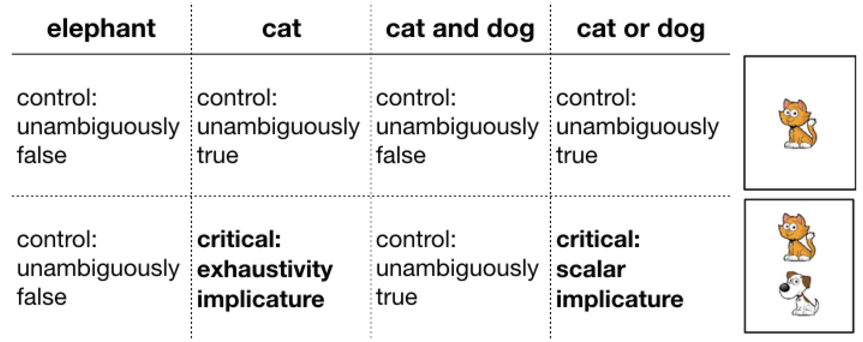
\includegraphics{writeup_files/figure-latex/trials-1} 

}

\caption{Trial types represented by example cards and guesses.}\label{fig:trials}
\end{figure}

\subsection{Procedure}\label{procedure}

\subsection{Pre-registered Analysis}\label{pre-registered-analysis}

This study set out to test the hypothesis that the proportion of
pragmatic vs.~literal responses in a truth values judgement task changes
based on the number of response options available to the participants.
We test this hypothesis formally using a binomial mixed effects model
with the fixed effect of blah and the random effects of blah.

\begin{verbatim}
## implicature_rate ~ response_type + (1 + response_type | tiral_type) + 
##     (1 | participant)
\end{verbatim}

\section{Results}\label{results}

\section{Analysis}\label{analysis}

\section{Modeling}\label{modeling}

\section{Discussion}\label{discussion}

\newpage

\section{References}\label{references}

\setlength{\parindent}{-0.5in} \setlength{\leftskip}{0.5in}






\end{document}
